\section{Number of Co atoms in each composition}
\label{sec:Cluster_configuration}

In Table \ref{tab:cluster} we enumerate the total number of Co atoms in the 15-atom cluster that corresponds to each alloy concentration ($N_{\textnormal{Co}}$), as well as the maximum/minimum number of Co atoms that can be placed within the nearest neighboring shell ($n_{\textnormal{max}}$ and $n_{\textnormal{min}}$ in their Co-centered configurations, respectively -- see Section \ref{subsec:clusters} for definitions).


\section{ASD simulations $J_{ij}$ parameters}
\label{sec:jijs-sets-asd}

Figure \ref{fig:embedded-cluster-jij} depicts the $J_{ij}$ parameters used to obtain the atomistic spin dynamics (ASD) results of Section \ref{sec:explicit-asd}. The plots correspond to the computed $J_{ij}$ values for each of the Fe and Co atoms of the embedded cluster of Fig. \ref{fig:cluster-example} taken as the reference site, as well as for the Fe$_{87}$Co$_{13}$ VCA (\textit{Inset}, in gray).

\begin{figure}[!htb]
        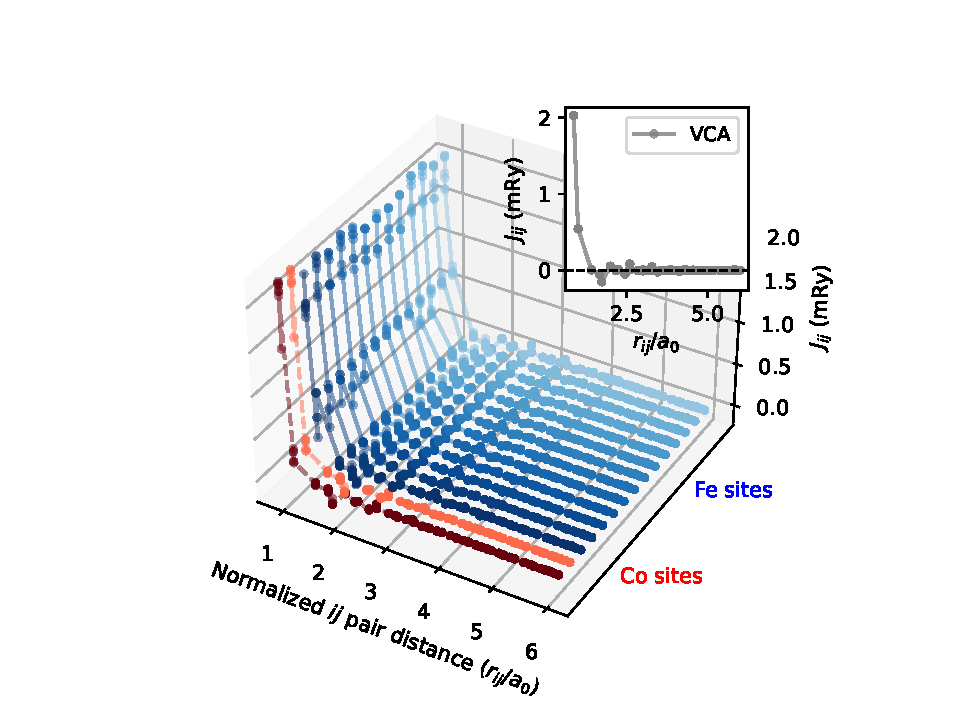
\includegraphics[width=\columnwidth]{Fig9.pdf} 
        \caption{Calculated Heisenberg exchange interaction parameters for each Fe (shades of blue) or Co (shades of red) atom within the embedded cluster illustrated in Fig. \ref{fig:cluster-example}, with each atom taken as a reference site.  The \textit{Inset} highlights, in gray, the $J_{ij}$ parameters computed for the VCA Fe$_{87}$Co$_{13}$. Lines are guides for the eyes.}
        \label{fig:embedded-cluster-jij} 
\end{figure}


\begin{table*}[htb]
\Large
\caption{\label{tab:cluster}
The total number of Co atoms ($N_{\textnormal{Co}}$) and the maximum (minimum) amount of Co in the nearest-neighborhood $n_{\textnormal{max}}$ ($n_{\textnormal{min}}$) within the cluster and in each composition. All these clusters refer to Co-centered configurations.}

\begin{ruledtabular}
\resizebox{0.5\textwidth}{!}{
\begin{tabular}{cccccc}
\multicolumn{1}{c}{}&
\multicolumn{1}{c}{Composition} & {$N_{\textnormal{Co}}$} & $n_{\textnormal{max}}$ & $n_{\textnormal{min}}$&\\
\colrule \\
{}&Fe & 0 & 0 &0\\
{}&Fe$_{87}$Co$_{13}$ & 2 & 1&0\\ 
{}&Fe$_{80}$Co$_{20}$ & 3 & 2&0\\ 
{}&Fe$_{74}$Co$_{26}$ & 4 & 3&0\\ 
{}&Fe$_{60}$Co$_{40}$ & 6 & 5&0\\ 
{}&Fe$_{53}$Co$_{47}$ & 7 & 6&0\\ 
{}&Fe$_{40}$Co$_{60}$ & 9 & 8&2\\
\end{tabular}
}
\end{ruledtabular}
\end{table*}


\section{Convergence of off-diagonal damping terms}
\label{sec:off-diagonal-convergence}

Figure \ref{fig:off-diag-sqs} shows the comparison of $\alpha^{\textnormal{eff}}_{xy}$ and $\alpha^{\textnormal{eff}}_{yx}$ with the diagonal terms, as well as their asymmetry $\left(\frac{\alpha^{\textnormal{eff}}_{xx}}{\alpha^{\textnormal{eff}}_{yy}}\right)$. 

\begin{figure}[!htb]
        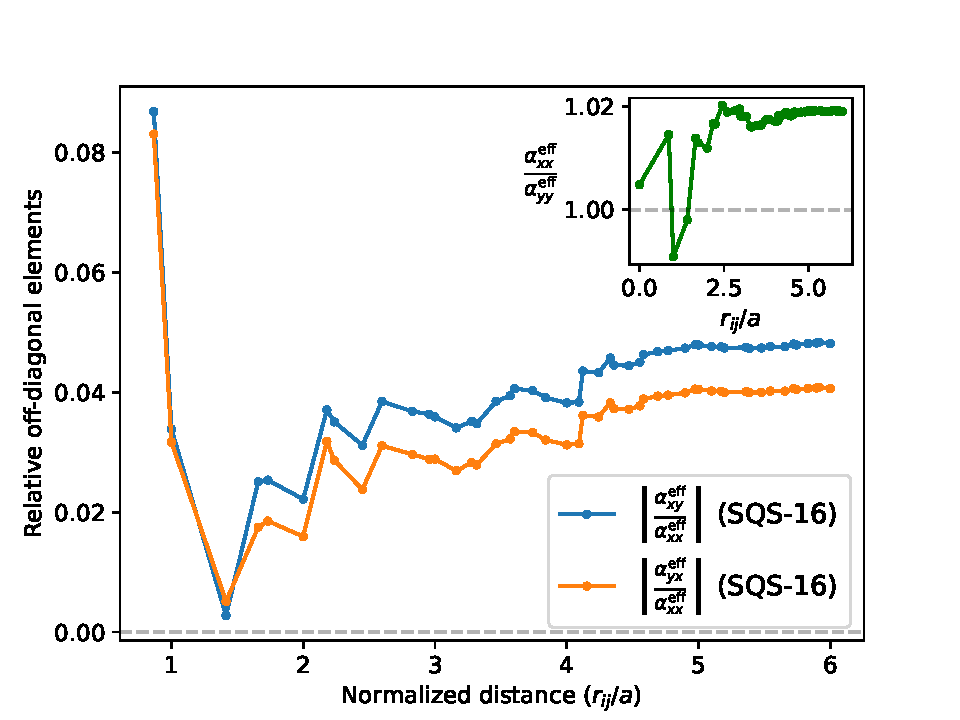
\includegraphics[width=\columnwidth]{Fig10.pdf} 
        \caption{Relative values of the off-diagonal terms $\alpha^{\textnormal{eff}}_{xy}$ (blue dots) and $\alpha^{\textnormal{eff}}_{yx}$ (orange dots) in the damping tensor $\hat{\alpha}^{\textnormal{eff}}$ for a SQS-16 cell of bcc Fe$_{50}$Co$_{50}$. The values were obtained using the formulation of Eq. \ref{eq:effective-tensor-elements}. \textit{Inset}: asymmetry between the diagonal terms $\alpha^{\textnormal{eff}}_{xx}$ and $\alpha^{\textnormal{eff}}_{yy}$, defined as $\frac{\alpha^{\textnormal{eff}}_{xx}}{\alpha^{\textnormal{eff}}_{yy}}$. The lines are guides for the eyes.}
        \label{fig:off-diag-sqs} 
\end{figure}


\section{VCA approach in FeCo systems}\label{VCA}
In the proposed EC-VCA model, the VCA was used to describe the external (non-explicit) medium. Despite its simple nature, the VCA approach has been demonstrated to be a reasonably valid method for investigating the properties of Fe$_x$Co$_{1-x}$ alloys. This has been discussed in the context of: (\textit{i}) magnetic moments (both spin and orbital) as corroborated by the replication of the well-known Slater-Pauling curve (see Fig. \ref{fig:Slater-Pauling}) \cite{PhysRevB.45.12911,PhysRevB.74.104422}; (\textit{ii}) transport properties \cite{PhysRevB.88.104408}; (\textit{iii}) a \textit{qualitatively} correct behavior of the magnetic anisotropy energy, as discussed in Refs. \cite{PhysRevB.89.144403,Neise2011,PhysRevB.86.174430,PhysRevB.93.224425}; and (\textit{iv}) a \textit{qualitatively} accurate trend of the total intrinsic Gilbert damping, as shown in Ref. \cite{PhysRevB.108.014433}, for which VCA is able to capture the remarkable low value at $\sim20-30\%$ of Co concentration, physically attributed to a pronounced minimum in the density of states at the Fermi level \cite{Schoen2016}. Although a non-negligible disorder is present in the spin-minority channel of bcc FeCo alloys \cite{PhysRevB.86.174430,PhysRevB.49.3352}, in an effective picture (in the context of Eq. \ref{eq:kambersky}), the average density of states of an explicit supercell is well reproduced by VCA \cite{PhysRevB.108.014433}. This trend, initially obtained via CPA analysis \cite{PhysRevLett.107.066603,PhysRevB.87.014430,PhysRevB.92.214407}, was later confirmed by experiments \cite{Schoen2016}.

\begin{figure}[!htb]
        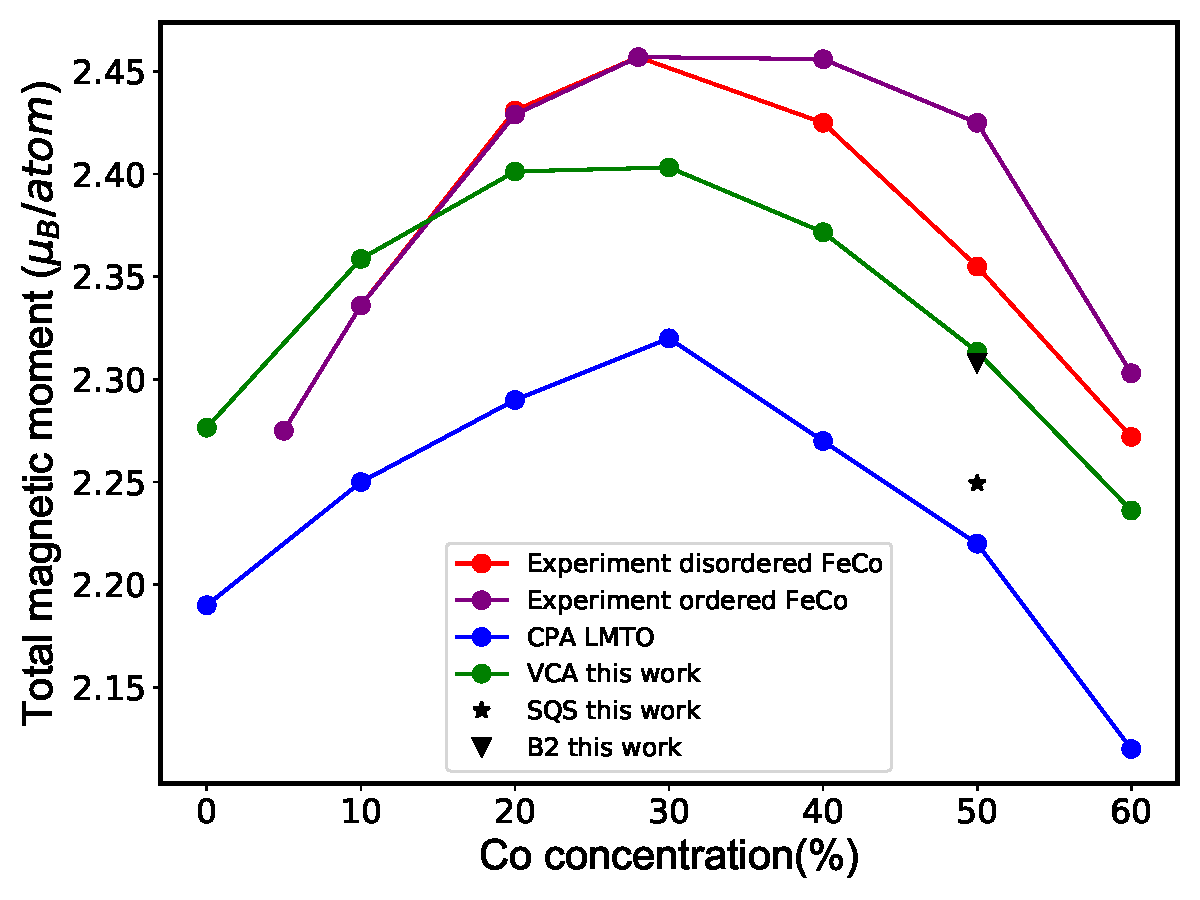
\includegraphics[width=\columnwidth]{Fig11.pdf} 
        \caption{Total magnetic moments (spin + orbital) as a function of the Co concentration, obtained for the FeCo alloys, exhibiting the well-known Slater-Pauling behavior. The calculations in this work are performed using 3 different models: VCA (green circles), SQS-16 (black star), and ordered B2 structure (black triangle). The blue dots represent the data obtained by using the CPA-LMTO method (extracted from Ref. \cite{PhysRevB.59.419}). Experimental data from Ref. \cite{Bardos1969} are depicted by the red and purple circles, representing the measurements for disordered and ordered FeCo alloys, respectively. Lines are guides for the eyes.} 
       
        \label{fig:Slater-Pauling} 
\end{figure}

 To give a more comprehensive relation between VCA, CPA and experimental results, we present a comparison of the Curie temperature ($\rm T_C$), spin wave stiffness ($\rm D_{ex}$) and Gilbert damping of Fe and Fe$_{1-x}$Co$_{x}$ alloys in Tables \ref{table1}-\ref{table3}. We found that the $T_C$, $\rm D_{ex}$ and dampings obtained from VCA and CPA show a good agreement, with acceptable discrepancies comparing to experiments.
\begin{table}[h!]
\caption{\label{table1}
The Curie temperature ($\rm T_C$) of the pure bcc Fe and Fe$_{1-x}$Co$_{x}$ alloys. In this work, whenever $x>0$, the electronic structure (and derived magnetic parameters) are calculated considering the VCA approach. The Curie temperature is evaluated from mean-field approximation ($\rm T_{C}^{MFA}$), random phase approximation  ($\rm T_{C}^{RPA}$), and Monte Carlo simulations  ($\rm T_{C}^{MC}$). For comparison, the theoretical and experimental value of $\rm T_C$ is shown. In other theoretical works, the CPA approach is adopted. } 
\resizebox{\columnwidth}{!}{
\begin{tabular}{ccccccc}

\hline
\hline
\multicolumn{4}{c}{This work}&\multicolumn{2}{c}{Other works}\\
\hline
\multicolumn{1}{c}{}&
\multicolumn{1}{c}{$\rm T_{C}^{MFA}$(K)}& $\rm T_{C}^{RPA}$(K) &$\rm T_C^{MC}$(K)& Expt. & Theory\\
\hline
bcc Fe  & 1274 & 919 & 960 &1044\cite{campbell1982ferromagnetic}  & 900$-$1238\cite{PhysRevLett.77.334,PhysRevB.55.14975,PhysRevB.75.054402,levzaic2007first,PhysRevB.95.184432}\\

bcc Fe$_{90}$Co$_{10}$  & 1712 & 1086 & 1300 &1164\cite{nishizawa1984co}& 1069\cite{PhysRevB.104.024403}\\

bcc Fe$_{80}$Co$_{20}$  & 2064 & 1426 & 1570 & 1225\cite{nishizawa1984co} & 1369\cite{PhysRevB.104.024403}\\

bcc Fe$_{70}$Co$_{30}$  & 2256 & 1667 & 1740  & $\sim1260$\cite{nishizawa1984co,karipoth2013synthesis}& 1490$-$1656\cite{levzaic2007first,PhysRevB.95.184432,PhysRevB.104.024403} \\

bcc Fe$_{60}$Co$_{40}$  & 2304 & 1790 & 1800 & 1268\cite{nishizawa1984co}& 1547\cite{PhysRevB.104.024403}\\

bcc Fe$_{50}$Co$_{50}$  & 2230 & 1782 & 1780 &  1253$–$1370\cite{nishizawa1984co,kawahara2003high} &1568$-$1634\cite{PhysRevB.104.024403,levzaic2007first,PhysRevB.95.184432} \\

bcc Fe$_{40}$Co$_{60}$  & 2067 & 1670 & 960& 1211\cite{karipoth2013synthesis}& $-$\\
\hline
\hline

\end{tabular}

}
\end{table}



\begin{table}[h!]

\caption{\label{table2}
The comparison of exchange stiffness ($\rm D_{ex}$) in this work and other works for the pure bcc Fe and Fe$_{1-x}$Co$_{x}$ alloys. } 
\resizebox{\columnwidth}{!}{
\begin{tabular}{cccc}
\hline
\hline
\multicolumn{1}{c}{}&This work&\multicolumn{2}{c}{Other works}\\
\hline
\multicolumn{1}{c}{}&
$\rm D_{ex}$ (meV$\cdot$\AA$^{2}$) & Expt. & Theory \\
\hline \\
bcc Fe  &  290 & 266$-$314\cite{stringfellow1968observation,PhysRevB.7.336,PhysRevLett.15.146} &247$-$410\cite{PhysRevB.55.14975,PhysRevB.104.024403}\\

bcc Fe$_{90}$Co$_{10}$  & 330 & 
$\sim345$ \cite{PhysRevLett.14.698} &
405\cite{PhysRevB.104.024403}\\

bcc Fe$_{80}$Co$_{20}$  & 411 & 
$\sim360$ \cite{PhysRevLett.14.698}
& 477\cite{PhysRevB.104.024403}\\

bcc Fe$_{70}$Co$_{30}$  & 493 & $\sim410$$-$470\cite{liu1994exchange,PhysRevLett.14.698} & 567\cite{PhysRevB.104.024403}\\

bcc Fe$_{60}$Co$_{40}$  & 561 &$\sim445$$-$530\cite{liu1994exchange,PhysRevLett.14.698} & 624\cite{PhysRevB.104.024403}\\

bcc Fe$_{50}$Co$_{50}$  & 592 &800\cite{liu1994exchange} &526$-$677\cite{PhysRevB.95.184432,PhysRevB.104.024403} \\

bcc Fe$_{40}$Co$_{60}$  & 578 
& $\sim480$ \cite{PhysRevLett.14.698}
&466\cite{PhysRevB.95.184432}\\
\hline
\hline
\end{tabular}
}
\end{table}



\begin{table}[h!]
\caption{\label{table3}
 The comparison of damping ($\alpha$) in this work and other works for the pure bcc Fe and Fe$_{1-x}$Co$_{x}$ alloys. } 
 \resizebox{\columnwidth}{!}{
 \begin{tabular}{cccc}
\hline
\hline

\multicolumn{1}{c}{}&This work&\multicolumn{2}{c}{Other works}\\
\hline
\multicolumn{1}{c}{}&
$\rm \alpha$ ($\times10^{-3}$) & Expt. & Theory \\
\hline \\
bcc Fe  &  2.1 &1.9$-$7.2\cite{Schoen2016,Oogane2006,PhysRevB.87.014430,PhysRevLett.124.157201, PhysRevLett.98.117601,PhysRevB.10.179,PhysRevB.18.4856,PhysRevB.95.134411}&1.3$-$3.2\cite{PhysRevB.87.014430,PhysRevLett.99.027204,Hiramatsu2021} \\

bcc Fe$_{90}$Co$_{10}$  & 1.4 &1.2\cite{Schoen2016} &0.5$-$0.8\cite{PhysRevB.92.214407,PhysRevB.87.014430, PhysRevB.98.104406} \\

bcc Fe$_{80}$Co$_{20}$  & 1.0 &  0.8\cite{Schoen2016}&0.4$-$0.6\cite{PhysRevB.92.214407,PhysRevB.87.014430,PhysRevB.98.104406}\\

bcc Fe$_{70}$Co$_{30}$ & 0.9 & 0.5$-$1.7\cite{Schoen2016, Oogane2006,Lee2017}&0.5$-$0.8\cite{PhysRevB.92.214407,PhysRevB.87.014430} \\

bcc Fe$_{60}$Co$_{40}$  & 1.1  & $\sim1.1$\footnote{bcc Fe$_{65}$Co$_{35}$ \cite{PhysRevB.95.134411}} & 0.8$-$1.1\cite{PhysRevB.92.214407,PhysRevB.87.014430,PhysRevB.98.104406}\\

bcc Fe$_{50}$Co$_{50}$  & 1.6 & 2.0$-$3.2\cite{Schoen2016, Oogane2006,PhysRevLett.122.117203} & 1.0$-$1.3\cite{PhysRevB.92.214407,PhysRevB.87.014430,PhysRevB.98.104406}\\

bcc Fe$_{40}$Co$_{60}$  & 1.6 &1.3$-$2.5\cite{Schoen2016}&1.6\cite{PhysRevB.92.214407,PhysRevB.87.014430} \\
\hline
\hline
\end{tabular}

}
\end{table}





\section{ Effective damping  }
\label{sec:damping_formula}
As mentioned in Section \ref{sec:methods}, in the FMR experiments the magnetic moments are excited in a coherent mode. Thus, a macrospin description with the summed total effective magnetization $\vec{M}^{\textnormal{eff}}_i$ reads

\begin{equation}\label{eq:sum-damping}
\begin{split}
\vec{M}^{\textnormal{eff}}_i =\sum_i \vec{M}_i.
\end{split}
\end{equation}

The dynamics of this macrospin is well described by the Landau-Lifshitz-Gilbert equation 

\begin{equation}\label{eq:llg-meff}
\frac{\partial \vec{M}^{\textnormal{eff}}}{\partial t}=\vec{M^{\textnormal{eff}}}\times\left(-\gamma\vec{B}+\frac{\alpha^{\textnormal{eff}}}{\left|\vec{M}^{\textnormal{eff}}\right|} \frac{\partial \vec{M}^{\textnormal{eff}}}{\partial t}\right),
\end{equation}

\noindent where $\gamma$ is the gyromagnetic ratio, $\vec{B}$ is the effective field acting on the macrospin and $\left|\vec{M}^{\textnormal{eff}}\right|=\left|\sum_i\vec{m}_i\right|\leq\sum_i\left|\vec{m}_{i}\right|$. Since we aim to describe a coherent motion of the individual spins, i.e., a ferromagnetic collinear state at all times $t$, by construction we have $\left|\vec{M}^{\textnormal{eff}}\right|=\sum_i\left|\vec{m}_{i}\right|$  and $\vec{B}$ isotropic with respect to all atomic sites $i$ ($\vec{B}_i=\vec{B}$). A general form of LLG equation incorporating the non-local damping (first assuming it to be a scalar parameter) is:

\begin{equation}\label{eq:llg_nonlocal}
\frac{\partial \vec{m}_i}{\partial t}=\vec{m}_i\times\left(-\gamma \left[\vec{B}_i+\vec{b}_i(t)\right]+\sum_j\frac{\alpha_{ij}}{m_j}\frac{\partial \vec{m}_j}{\partial t}\right).
\end{equation}

Working with Eq. \ref{eq:llg-meff} we have:

\begin{align}\label{eq:meff-deduction}
\frac{\partial \vec{M}^{\textnormal{eff}}}{\partial t}
&=\sum_i \frac{\partial \vec{m}_i}{\partial t} \nonumber\\
&=\sum_i\left[\vec{m}_i\times(-\gamma \vec{B}_i+\sum_j\frac{\alpha_{ij}}{m_j} \frac{\partial \vec{m}_j}{\partial t} )\right] \nonumber\\
&=-\gamma \left[\sum_i\vec{m}_i\right]\times \vec{B}+\left[\sum_i{\vec{m}_i}\right]\times \left[\sum_j\frac{\alpha_{ij}}{m_j}\frac{\partial \vec{m}_j}{\partial t}\right].
\end{align}

Therefore, in the FMR regime, one can compare Eqs. \ref{eq:llg-meff} and \ref{eq:meff-deduction}, resulting in 

\begin{equation}\label{eq:comparison}
\vec{M}^{\textnormal{eff}} \times \frac{\alpha^{\textnormal{eff}}}{\left|\vec{M}^{\textnormal{eff}}\right|}\frac{\partial \vec{M}^{\textnormal{eff}}}{\partial t}  = \sum_i\vec{m}_i\times\sum_j \frac{\alpha_{ij}}{m_j} \frac{\partial \vec{m}_j}{\partial t} . 
\end{equation}

Let us write $\vec{M}^{\textnormal{eff}} = \left|\vec{M}^{\textnormal{eff}}\right|\vec{e}^{\textnormal{eff}} $ and $\vec{m}_i = \left|\vec{m}_i\right|\vec{e}_i$, where $\vec{e}^{\textnormal{eff}}$ and $\vec{e}_i$ are the spin moment orientation of the macrospin and the atomic spin at site $i$, respectively, at a given time $t$. Since we describe a coherent precession, then it is straightforward that $\frac{\partial \vec{e}_i}{\partial t}=\frac{\partial \vec{e}^{\textnormal{eff}}}{\partial t}$ and $\vec{e}_i=\vec{e}^{\textnormal{eff}}$. Hence, by Eq. \ref{eq:comparison}, we obtain 

\begin{align}\label{eq:effective-alpha-parameter}
\alpha^{\textnormal{eff}}&=\frac{1}{M^{\textnormal{eff}}}\sum_{ij} \left|\vec{m}_i \right|\alpha_{ij} \nonumber \\ 
&= \frac{1}{\sum_i \left|\vec{m}_i \right| } \sum_{ij} \left|\vec{m}_i \right|\alpha_{ij} = \frac{1}{\sum_i \left|\vec{m}_i \right| } \sum_{i}\left|\vec{m}_i \right|\alpha_i.
\end{align}

Here, we define the effective damping of spin moment $i$ as $\alpha_i=\sum_j{\alpha_{ij}}$ \cite{PhysRevB.108.014433}. For the general case where the Gilbert damping is expressed as a tensor $\boldsymbol{\alpha}_{ij}$, it becomes harder to disentangle a closed form for $\alpha^{\textnormal{eff}}$, and the effective damping parameter should be extracted directly from simulations containing the explicit $\boldsymbol{\alpha}_{ij}$ expression. However, if we assume that the macrospin is also subjected to an effective damping in the tensor form, as suggested by previous works (e.g., Ref. \cite{PhysRevB.72.064450,PhysRevB.84.172403}), so that the term $\frac{\alpha^{\textnormal{eff}}}{\left|\vec{M}^{\textnormal{eff}}\right|}\frac{\partial \vec{M}^{\textnormal{eff}}}{\partial t}$ is replaced by $\frac{\boldsymbol{\alpha}^{\textnormal{eff}}}{\left|\vec{M}^{\textnormal{eff}}\right|}\cdot\frac{\partial \vec{M}^{\textnormal{eff}}}{\partial t}$, then for each element of $\boldsymbol{\alpha}^{\textnormal{eff}}$ we have

\begin{equation}
\label{eq:effective-tensor-elements}
\alpha^{\textnormal{eff}}_{\mu\nu} = \frac{1}{M^{\textnormal{eff}}}\sum_{ij} \left|\vec{m}_i \right|\alpha_{ij}^{\mu\nu},
\end{equation}


\noindent where $\mu,\nu\in\{x,y,z\}$. This result can be derived by applying the same reasoning of Eqs. \ref{eq:meff-deduction}-\ref{eq:effective-alpha-parameter}, however considering that both effective and atomistic LLG equations assume the general form of a tensorial Gilbert damping ($\boldsymbol{\alpha}^{\textnormal{eff}}$ and $\boldsymbol{\alpha}_{ij}$).






